
% \shorthandoff{;} with babel french
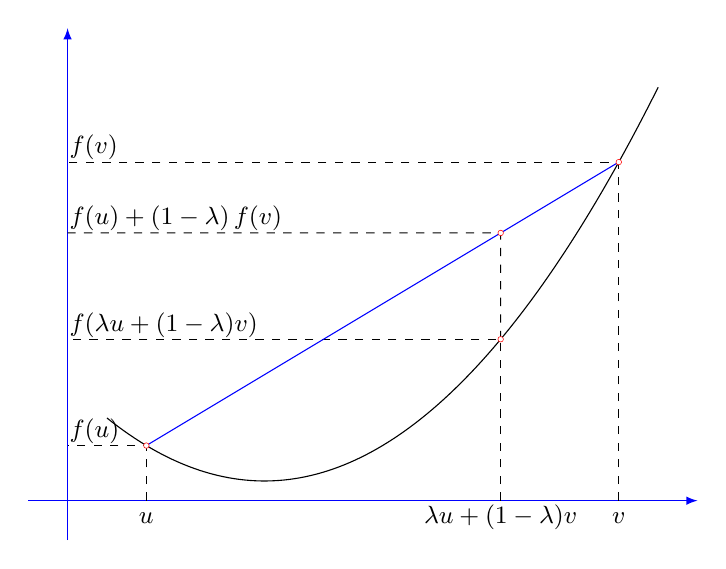
\begin{tikzpicture}[declare function={f(\x)=(\x-1)*(\x-1)/2 + 0.1;},x={(2.5cm,0)},y={(0,2.5cm)},samples=101,font=\small,inner sep=0.5pt]
  \draw[blue,-latex] (-0.2,0) -- (3.2,0);
  \draw[blue,-latex] (0,-0.2) -- (0,2.4);
  \coordinate (O) at (0,0);
  \draw plot[domain=0.2:3,variable=\x] ({\x},{f(\x)});
  \foreach [count=\Z] \X/\Y in {0.4/{u},2.2/{\lambda u +(1-\lambda) v},2.8/{v}}
  {\draw[dashed] (\X,0) coordinate (X\Z) node[below]{$\strut\Y$} -- (\X,{f(\X)}) coordinate (F\Z)
    -- (0,{f(\X)}) node[above right]{$f(\Y)$};}
  \draw[blue] (F1) -- (F3);
  \draw[dashed] (F2) --
  (intersection cs:first line={(X2)--(F2)}, second line={(F1)--(F3)})
  coordinate (F4) -- (O|-F4) node[above right]{$f(u)+(1-\lambda)\,f(v)$};
  \foreach \X in {1,...,4}
  {\draw[very thin,red,fill=white] (F\X) circle(1pt);}
\end{tikzpicture}
  